\section{Fundamentos de los sistemas difusos.}

\subsection{Introducción}
Desde su aparición en la década de los 60's hasta nuestros días, las
aplicaciones de la Lógica Difusa se han ido consolidando, paulatinamente al
comienzo, y con un desbordado crecimiento en los últimos cinco años.

 Se
encuentran en soluciones a problemas de control industrial, en predicción de
series de tiempo, como metodologías de archivo y búsqueda de Bases de
Datos, en Investigación Operacional, en estrategias de mantenimiento
predictivo y en otros campos más.
Las principales razones para tal proliferación de aplicaciones quizás sean la
sencillez conceptual de los Sistemas basados en Lógica Difusa, su facilidad
para adaptarse a casos particulares con pocas variaciones de parámetros,
su habilidad para combinar en forma unificada expresiones lingüísticas con
datos numéricos, y el no requerir de algoritmos muy sofisticados para su
implementación.



Es bien conocido que la teoría de conjuntos, el álgebra booleana y la lógica
tradicional son isomorfas\footnote{\url{http://matematica.laguia2000.com/general/isomorfismo}}, bajo transformaciones adecuadas. Esto significa
que tienen una estructura subyacente similar, y que por tanto las
definiciones que se hagan en una cualquiera de las tres teorías se puede
llevar a las otras dos, mediante transformaciones adecuadas. La \tableref{table:1}
muestra la correspondencia de algunos operadores.


\begin{table}[h]
	\centering
	\begin{tabular}{@{}ccc@{}}
		\toprule
		\multicolumn{1}{l}{\textbf{Teoría de conjuntos}} & \multicolumn{1}{l}{\textbf{Álgebra booleana}} & \multicolumn{1}{l}{\textbf{Lógica tradicional}} \\ \midrule
		\multicolumn{1}{c}{Intersección}               & \multicolumn{1}{c}{Conjunción}               & \multicolumn{1}{c}{AND}                        \\ \midrule
		\multicolumn{1}{c}{Unión}                      & \multicolumn{1}{c}{Disyunción}               & \multicolumn{1}{c}{OR}                         \\ \midrule
		Complemento                                      & Negación                                      & NOT                                             \\ \bottomrule
	\end{tabular}
	\caption{Correspondencia entre operadores de la Teoría de Conjuntos, el Álgebra Booleana y la Lógica Tradicional.}
	\label{table:1}
\end{table}

\subsection{Teoría de conjuntos difusos}
Una buena estrategia para presentar la teoría de Conjuntos Difusos,
consiste en recordar algunos aspectos de la teoría de conjuntos
convencionales (que llamaremos conjuntos concretos), y a partir de allí
hacer una extensión a los conjuntos difusos:

Un conjunto concreto se define como una colección de elementos que
existen dentro de un Universo. Así, dado el universo U que consta de los números enteros no negativos menores que 10:

\texttt{U = \{0,1,2,3,4,5,6,7,8,9\}}

podemos definir algunos conjuntos como\\
\newline
\null\hspace{0.59cm}\texttt{A = \{0,2,4,6,8\}},\newline
\null\hspace{0.37cm}\texttt{ B=\{1,3,5,7,9\}},\newline
\null\hspace{0.37cm}\texttt{ C=\{1,4,7\}} \ldots

En este ejemplo hemos establecido a qué conjuntos pertenece cada uno de los elementos del universo \texttt{U}, por lo tanto, cada conjunto podría definirse completamente por una función de pertenencia (\texttt{u(x)}) que opera sobre los elementos de dicho Universo, asignándole a cada uno un valor de 1 si pertenece o 0 si no pertenece al conjunto.

Tomemos como ejemplo el conjunto \texttt{C} del ejemplo anterior.
La función de pertenencia que lo define sería:
\\ \newline
\null\hspace{0.59cm}\texttt{u\textsubscript{C}(0)} = 0;\\
\null\hspace{0.59cm}\texttt{u\textsubscript{C}(1)} = 1;\\
\null\hspace{0.59cm}\texttt{u\textsubscript{C}(2)} = 0;\\
\null\hspace{0.59cm}\texttt{u\textsubscript{C}(3)} = 0;\\
\null\hspace{0.59cm}\texttt{u\textsubscript{C}(4)} = 1;\\
\null\hspace{0.59cm}\texttt{u\textsubscript{C}(5)} = 0;\\
\null\hspace{0.59cm}\texttt{u\textsubscript{C}(6)} = 0;\\
\null\hspace{0.59cm}\texttt{u\textsubscript{C}(7)} = 1;\\
\null\hspace{0.59cm}\texttt{u\textsubscript{C}(8)} = 0;\\
\null\hspace{0.59cm}\texttt{u\textsubscript{C}(9)} = 0;

Pues bien, un Conjunto Difuso se define de forma similar, con una
diferencia conceptual importante: un elemento puede pertenecer
parcialmente a un conjunto. De esta forma, un conjunto difuso D definido
sobre el mismo universo U puede ser el siguiente:
\\ \newline
\null\hspace{0.59cm}\texttt{C=\{20\%/1,50\%/4,100\%/7\}}\footnote{El símbolo ``/'' no significa ``dividido por'', simplemente es una cuestión de notación.}

La definición anterior significa que el elemento 1 pertenece en un 20\% al
conjunto \texttt{C} (y por tanto pertenece en un 80\% al complemento de \texttt{C}), en tanto
que el elemento 4 pertenece en un 50\%, y el elemento 7 en un 100\% .

De forma alternativa, diríamos que la función de pertenencia \texttt{u\textsubscript{C}(x)} del
conjunto D es la siguiente:
\\ \newline
\null\hspace{0.59cm}\texttt{u\textsubscript{C}(0)} = 0.0;\\
\null\hspace{0.59cm}\texttt{u\textsubscript{C}(1)} = 0.2;\\
\null\hspace{0.59cm}\texttt{u\textsubscript{C}(2)} = 0.0;\\
\null\hspace{0.59cm}\texttt{u\textsubscript{C}(3)} = 0.0;\\
\null\hspace{0.59cm}\texttt{u\textsubscript{C}(4)} = 0.5;\\
\null\hspace{0.59cm}\texttt{u\textsubscript{C}(5)} = 0.0;\\
\null\hspace{0.59cm}\texttt{u\textsubscript{C}(6)} = 0.0;\\
\null\hspace{0.59cm}\texttt{u\textsubscript{C}(7)} = 1.0;\\
\null\hspace{0.59cm}\texttt{u\textsubscript{C}(8)} = 0.0;\\
\null\hspace{0.59cm}\texttt{u\textsubscript{C}(9)} = 0.0;

Aquí podemos ver las primeras diferencias entre los Conjuntos Concretos y los Conjuntos Difusos, entre las que cabe destacar:
\begin{itemize}
	\item La función de pertenencia asociada a los conjuntos concretos sólo puede
	tener dos valores: 1 ó 0, mientras que en los conjuntos difusos puede
	tener cualquier valor entre 0 y 1.
	\item Un elemento puede pertenecer (parcialmente) a un conjunto difuso y
	simultáneamente pertenecer (parcialmente) al complemento de dicho
	conjunto. Esto no es posible en los conjuntos concretos, ya que
	constituiría una violación al \textit{principio del tercer excluido.}\footnote{\url{https://es.wikipedia.org/wiki/Principio_del_tercero_excluido}}
	\item Las fronteras de un conjunto concreto son exactas, en tanto que las de
	un conjunto difuso son, precisamente, difusas, ya que existen elementos
	en las fronteras mismas, y estos elementos están a la vez dentro y fuera
	del conjunto.
\end{itemize}

Pero, qué sentido puede tener el pertenecer parcialmente a un conjunto? En
muchos casos puede tener más sentido que pertenecer totalmente a un
conjunto; veamos un ejemplo:

\textit{Ejemplo 1:} Supóngase que se desea clasificar a los miembros de un equipo
de fútbol según su estatura en tres conjuntos, Bajos, Medianos y Altos.
Podría plantearse que se es Bajo si se tiene una estatura inferior a, por
ejemplo, 160 cm, que se es Mediano si la estatura es superior o igual a 160
cm e inferior a 180 cm, y se es alto si la estatura es superior o igual a 180
cm, con lo que se lograría una clasificación en conjuntos concretos. \label{ej:1}

Sin embargo, qué tan grande es la diferencia que existe entre dos jugadores
del equipo, uno con estatura de 179.9 cm y otro de 180.0 cm? Ese milímetro
de diferencia quizás no represente en la práctica algo significativo, y sin
embargo los dos jugadores han quedado rotulados con etiquetas distintas:
uno es Mediano y el otro es Alto. Si se optase por efectuar la misma
clasificación con conjuntos difusos estos cambios abruptos se evitarían,
debido a que las fronteras entre los conjuntos permitirían cambios graduales
en la clasificación.

\begin{figure}[H]
	\centering
	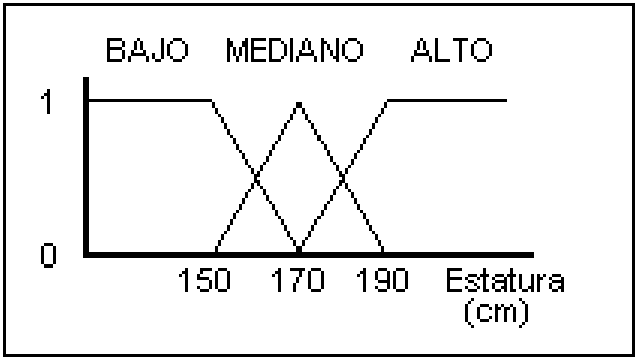
\includegraphics[scale=0.3]{images/fuzzy_example.png}
	\caption{Funciones de pertenencia del ejemplo 1}
	\label{fig:ej1}
\end{figure}
La \figureref{fig:ej1} muestra cómo podría hacerse tal clasificación: el universo de
discurso sería el conjunto continuo de todas las posibles estaturas (el
intervalo [130,210]cm por ejemplo).La forma de
estas funciones de pertenencia no debe ser necesariamente la de la figura 1,
pues depende de lo que se entienda por ``Bajo'', ``Mediano'' y ``Alto''.

\begin{figure}[H]
	\centering
	\begin{subfigure}[b]{0.4\textwidth}
		\centering
		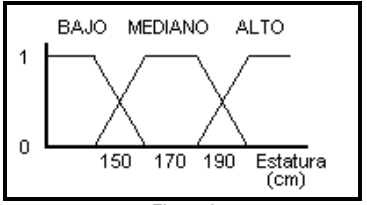
\includegraphics[scale = 0.5]{images/fuzzy_example_alt1.png}
		\caption{Representación alternativa del ejemplo 1}
		\label{fig:fuzzy1}
	\end{subfigure}
	~ %add desired spacing between images, e. g. ~, \quad, \qquad, \hfill etc. 
	%(or a blank line to force the subfigure onto a new line)
	\begin{subfigure}[b]{0.4\textwidth}
		\centering
		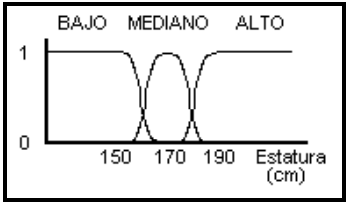
\includegraphics[scale = 0.5]{images/fuzzy_example_alt2.png}
		\caption{Representación alternativa del ejemplo 1}
		\label{fig:fuzzy2}
	\end{subfigure}
	\label{fig:alternativas}	
\end{figure}
En las \textit{figuras \ref{fig:fuzzy1} y \ref{fig:fuzzy2}} podemos ver otras alternativas para representar dichas funciones.

\subsection{Inferencia en lógica difusa}
La Inferencia lógica consiste en la combinación de proposiciones para
producir nuevas proposiciones. Así, al combinar la proposición \texttt{``X es A''} con
la proposición \texttt{``IF X es A THEN Y es B''}, se puede inferir la proposición \texttt{``Y es
B''} (ver figura \figureref{fig:inf})

\begin{figure}[H]
	\centering
	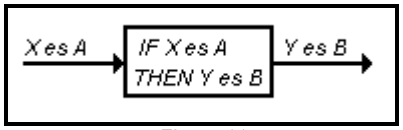
\includegraphics[scale=0.5]{images/logica_difusa.png}
	\caption{Inferencia en lógica tradicional.}
	\label{fig:inf}
\end{figure}

Una inferencia como ésta sólo es posible en
la lógica tradicional si la primera proposición \texttt{(``X es A'') }es idéntica a la
primera parte de la segunda proposición \texttt{(``(IF) X es A'')}; sin embargo, en la
lógica difusa estas dos proposiciones no necesariamente deben ser
idénticas, debido a que las fronteras de los conjuntos no son precisas. Así, al
combinar la proposición \texttt{``X es A*''} con la proposición \texttt{``IF X es A THEN Y es
B''}, puede obtenerse la proposición \texttt{``Y es B*''} (ver figura \figureref{fig:inf}).

\begin{figure}[H]
	\centering
	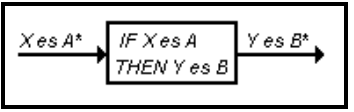
\includegraphics[scale=0.67]{images/logica_difusa_1.png}
	\caption{Inferencia en lógica difusa.}
	\label{fig:inf1}
\end{figure}

En la \figureref{fig:inferencia} podemos ver los mecanismos de Inferencia en Lógica Difusa \footnote{\url{http://www.cs.princeton.edu/courses/archive/fall07/cos436/HIDDEN/Knapp/fuzzy004.htm}}

\begin{figure}[H]
	\centering
	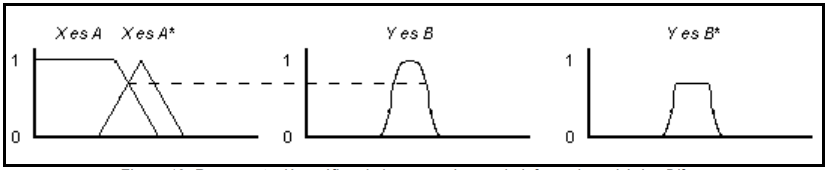
\includegraphics[scale=0.67]{images/mecanismos_inferencias_logica_difusa.png}
	\caption{Representación gráfica de los mecanismos de Inferencia en Lógica Difusa}
	\label{fig:inferencia}
\end{figure}

\subsection{Sistemas de lógica difusa}
Los mecanismos de Inferencia presentados en el numeral anterior permiten
obtener Conjuntos difusos a partir de la combinación de Conjuntos difusos
con reglas de la forma \texttt{IF... THEN...}; Un Sistema de Lógica Difusa aprovecha
esos mecanismos como el motor de cálculo de un sistema cuyas entradas y
salidas son números concretos.

En la \figureref{fig:sistemas_difusos} podemos ver la estructura básica de un Sistema de Lógica difusa.
El sistema recibe varias entradas numéricas y entrega varias salidas
numéricas. El bloque Difusor se encarga de convertir las entradas en
conjuntos difusos, que son entregados al bloque Máquina de Inferencia; este
bloque, apoyado en un conjunto de reglas de la forma \texttt{IF... THEN...}
almacenadas en la Base de Reglas, produce varios conjuntos difusos para
que el bloque Concresor los tome y los convierta en salidas numéricas
concretas.
\begin{figure}[H]
	\centering
	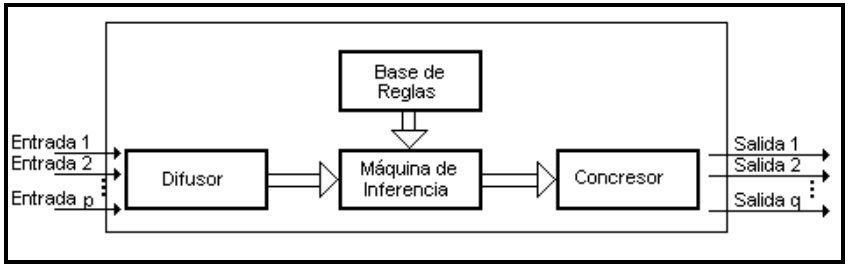
\includegraphics[scale=0.67]{images/sistemas_difusos.png}
	\caption{Estructura de un Sistema de Lógica Difusa}
	\label{fig:sistemas_difusos}
\end{figure}


Cada una de las variables de entrada y de salida tiene una representación
dentro del Sistema de Lógica Difusa en forma de Variables Lingüísticas. Una
variable lingüística tiene, entre otras cosas, una colección de atributos que
puede adquirir la variable, y cada atributo está representado por un conjunto
difuso. Así, retomando el ejemplo de la \figureref{fig:ej1}, la variable Estatura tendría
tres atributos, Bajo, Mediano y Alto, y cada uno de estos atributos estaría
representado por el conjunto difuso respectivo de la \figureref{fig:ej1}. Estos atributos
reciben el nombre de Valores Lingüísticos.